\documentclass{article} % The class file specifying the document structure

\usepackage[utf8]{inputenc} % Required for inputting international characters
\usepackage[T1]{fontenc} % Output font encoding for international characters

\usepackage{palatino} 
\usepackage{verbatim}


\usepackage[backend=bibtex]{biblatex} 
\addbibresource{references}

\usepackage{amsmath}
\usepackage{amsthm}
\usepackage{amssymb}
\usepackage{tikz}
\usetikzlibrary{positioning,shapes,arrows,matrix,fit,scopes}


\usepackage[autostyle=true]{csquotes} % Required to generate language-dependent quotes in the bibliography



\begin{document}

\begin{figure}[h!]
\centering
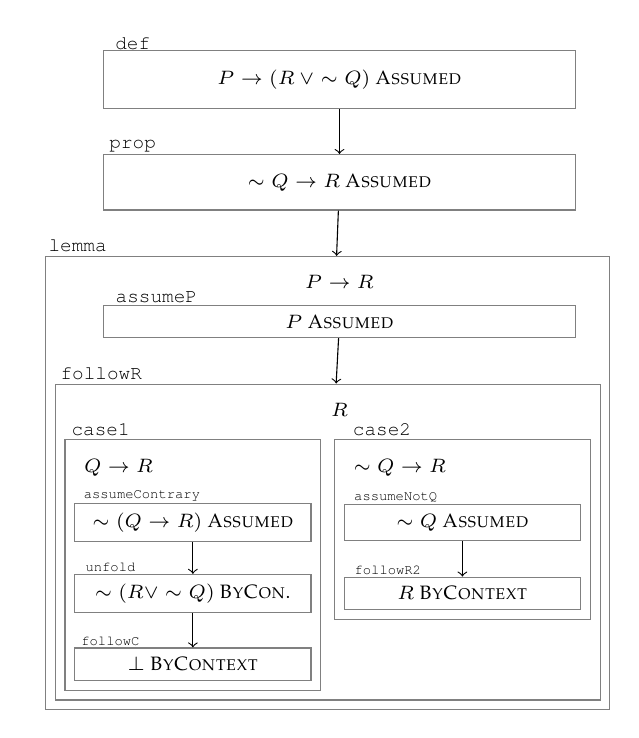
\begin{tikzpicture}[
  node distance=.5cm,
  title/.style={font=\scriptsize},
  typetag/.style={rectangle, draw=black!50, font=\scriptsize, anchor=west, minimum width=3cm}
]
	
\node (defC) [title, label={[xshift=-2.7cm, yshift=0.01cm]\scriptsize \texttt{ def}}] { $P \rightarrow (R \ \vee \sim Q)$ \textsc{Assumed}};
\node (def) [draw=black!50, fit={(defC)}, minimum width=6cm] {};
  
\node (def2C) [title, label={[xshift=-2.7cm, yshift=0.03cm]\scriptsize \texttt{ prop}}, below=.7cm of def] { $\sim Q \rightarrow R $  \textsc{Assumed}};
\node (def2) [draw=black!50, fit={(def2C)}, minimum width=6cm] {} edge[<-] (def);
  
\node (lemmaC) [title, label={[xshift=-3.4cm, yshift=0.05cm]\scriptsize \texttt{ lemma}}, below=.7cm of def2, minimum width=6cm] { $P \rightarrow R$ };

 		\node (assP) [below=of lemmaC.west, typetag, minimum width=6cm, label={[xshift=-2.4cm, yshift=-.1cm]\scriptsize \texttt{ assumeP}}] {$P$ \textsc{Assumed}};
 		
 		\node (followsRC) [below=.7cm of assP, label={[xshift=-3.1cm, yshift=0.05cm]\scriptsize \texttt{ followR}}, title, minimum width=5.6cm] {$R$};
 		
		  		\node (Q2RC) [title, label={[xshift=-.3cm, yshift=0.05cm]\scriptsize \texttt{ case1}}, below=.5cm of followsRC.west] {$Q \rightarrow R$};
		  				\node (assContrary) [below=.7cm of Q2RC.west, label={[xshift=-.7cm, yshift=-.1cm]\tiny \texttt{ assumeContrary}}, typetag] {$\sim (Q \rightarrow R)$ \textsc{Assumed}};
		  				\node (transform) [below=.9cm of assContrary.west, label={[xshift=-1.1cm, yshift=-.1cm]\tiny \texttt{ unfold}}, typetag] {$\sim (R  \vee \sim Q)$ \textsc{ByCon.}} edge[<-] (assContrary);
		  				\node (followsBot) [below=.9cm of transform.west, label={[xshift=-1.1cm, yshift=-.1cm]\tiny \texttt{ followC}}, typetag] {$\bot$ \textsc{ByContext}} edge[<-] (transform);
		  		 \node (Q2R) [draw=black!50, fit={(Q2RC) (assContrary) (transform) (followsBot)}] {};
		  
		  		\node (notQ2RC) [title, label={[xshift=-.3cm, yshift=0.05cm]\scriptsize \texttt{ case2}},right=2.3cm of Q2RC] {$\sim Q \rightarrow R$};
		  				\node (assQ) [below=.7cm of notQ2RC.west, label={[xshift=-.9cm, yshift=-.11cm]\tiny \texttt{ assumeNotQ}}, typetag] {$\sim Q$ \textsc{Assumed}};
		  				\node (followsGoal) [below=.9cm of assQ.west, label={[xshift=-1.0cm, yshift=-.1cm]\tiny \texttt{ followR2}}, typetag] {$R$ \textsc{ByContext}} edge[<-] (assQ);
		  		 \node (notQ2R) [draw=black!50, fit={(notQ2RC) (assQ) (followsGoal)}] {};
		
		\node (followsR) [draw=black!50, fit={(followsRC) (Q2R) (notQ2R)}] {} edge[<-] (assP);

\node [draw=black!50, fit={(lemmaC) (followsR)}] {} edge[<-] (def2);

\end{tikzpicture}
\label{figStatementSequence}
\end{figure}


\end{document}  
